\section{Architecture and API}
\begin{figure}[t]
% \vspace{-5pt}
\centering
 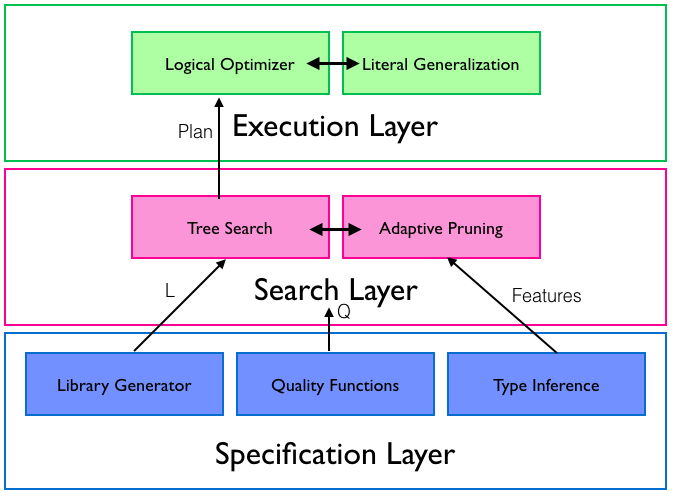
\includegraphics[width=\columnwidth]{figures/alphacleanarch.png}
 \caption{ \sys is given a specification of quality (e.g., integrity constraints or a statistical model the data must conform to) and a language  of  allowed  data  transformations,  and  it  searches  to find a sequence of transformations that maximizes the quality metric. \label{fig:arch} }
\end{figure}


This section describes the three major components of the \sys system architecture (\Cref{fig:arch}), split between the user interface to specify the cleaning problem, the core search algorithm, and optimization of the resulting cleaning program.  We focus on the interface and program optimization in this section, and focus on the search component and its optimizations in the rest of the paper.

The {\it Specification Interface} takes as input domain-specific cleanliness measures and data cleaning operations that the user provides  and translates them into a quality function and data transformation language.   For instance, our current implementation supports a wide range of quality functions including: attribute type constraints, functional dependencies, denial constraints, lookup tables~\cite{}, parametric and non-parametric outlier models, and correlations between numeric attributes.  Our existing cleaning data transformations primarily focus on conditional cell and record transformations that apply a transformation to all cells or records that satisfy a predicate; both the transformation parameters and the predicate are learned by \sys.  \Cref{s:appendix} provides a detailed description of the supported functions and extendible API. 

The {\it Search} component takes as input $Q$ and $L$, and performs a greedy search heuristic to find a program $p^* \in L$ that maximizes $Q$.  Users can supply hints that exploit the problem structure to reduce the runtime by pruning the search space and parallelizing the search.  \sys supports two main classes of pruning-based optimizations. {\it Static} rules that invalidate programs in $L$ that are unlikely to be useful.  For instance, composing the same idempotent transformation (e.g., \texttt{find\_replace(SFO, SF, city\_name)}) is redundant and can be immediately skipped.  {\it Dynamic} rules have access to the result of a candidate program when making pruning decisions, and we propose a novel approach to learn automatic dynamic pruning rules that can reduce end-to-end runtimes by up to \ewu{XXX} at the expense of slightly lower recall.  \Cref{s:search} describes the pruning rules and parallelization optimization in detail.


Finally, once search component outputs the cleaning program $p^*$, the {\it Program Optimizer} optimizes $P^*$ provides an API to apply simple query compilation techniques.  \sys currently replaces variables with literal values whenever possible.  In addition, we implement loop fusion~\cite{} to avoid scanning the input and intermediate relations for each transformation in $p^*$. Finally, we inline the data transformation functions into the loops.    

For example, consider the operations from~\Cref{ex3}.  Since the \texttt{find\_replace} operations do not conflict, it is inefficient to loop through over the relation instance three separate times.  
Since they do not conflict, it would be inefficient to execute them sequentially and iterate over the data three separate times.
Instead, one should combine the operations together and execute at once:
\begin{lstlisting}
for r in rows:
 if r[city_name] == `New York':
   r[city_name] = `New York City'
 elif r[city_name] == `San Francisc':
   r[city_name] = `San Francisco'
 if r[city_code] == `NYC'
   r[city_code] = `NY'
\end{lstlisting}
We find that even these simple optimizations improve the final program runtime by \ewu{XXX}, and leave further improvements to future work.


% The user can optionally provide custom quality functions and data transformations as simple Python class definitions.      takes as input user specifications of the quality function and data transformation language, alongside search configuration parameters.


\if{0}
Now, we will overview some of the preliminary concepts and describe how this formalism inspires a modular system API.
\sys is designed as a software stack with three layers: a specification layer, a search layer, and an execution layer.
To understand how these layers interact, we will use the example in Section 2 throughout this section.


\subsection{Specification Layer} The provides an API for specifying a quality function and a language of transformations. This allows one to specify a data cleaning problem for a particular dirty instance. As described in the previous section, we provide an API for translating common data cleaning specifications, constraints, statistical models, and gold standard examples, into quality functions. 

The harder problem is specifying the language. 
The challenge is that most data transformations are parametrized by literal values from the database.
We need efficient techniques to automatically enumerate this transformation set before we apply the search.
The language is generated through a transformation templates which are dynamically populated by literals in the database.
A template is a parametrized transformation:
\[T(R, [\theta_1, \theta_2,...,\theta_k] ): \mathcal{R} \mapsto  \mathcal{R},\] where the parameters $[\theta_i]$ are populated by literal values.
Each $\theta_i$ represents an SQL query except for special parameters such as attribute names and data-independent hyperparameters.
The system dynamically generates all possible literal instances of this transformation by taking the cartesian product of the query results.

In the running example, consider the following function:
\[
\textsf{find\_replace}(\text{source}, \text{target}, \text{attribute})
\]
\begin{lstlisting}
source := SELECT attribute from R;
target := SELECT attribute from R;
\end{lstlisting}
Likewise for numerical transformations, consider the function that clips outlier values outside 6 standard deviations of the mean:
\[
\textsf{clip}(\text{mean}, \text{threshold})
\]
\begin{lstlisting}
mean := SELECT mean(attribute) from R;
threshold := SELECT 6*std(attribute) from R;
\end{lstlisting}
\sys provides queries and filters for a number of common parametrizations or they can be specified manually.

\subsection{Search Layer (Section 5)} The next layer is the search layer, which implements the basic search algorithm of \sys. This algorithm is a distributed best-first greedy search.  
With no additional information, the search approach described would have to evaluate $61^3 = 226981$ transformations, which is clearly impractical even for this small example.
This layer also provides an interface for custom search optimizations:

\vspace{0.5em}\noindent\textbf{Static Optimizations: } A static optimization is a regular expression that all transformation sequences must satisfy independent of the data. 
\[\textsf{static\_opt}(L, \text{regex} ) \mapsto L'\]
For example, since the find-and-replace operations are idempotent, i.e., $T(T(R)) = T(R)$, we may want to only consider the set of all sequences with no neighboring repeated transformations. Similarly, we may also want to prune all search branches that make no effect (i.e., find-and-replace New York with New York).
These two regular expressions alone reduce the overall number of evaluations by $48\%$ in the above example (120050 v.s. 226981 evaluations).
There are several other possible optimizations  such as avoiding changes that reverse previous changes $T_i(T_j(R)) = R$.


\vspace{0.5em}\noindent\textbf{Dynamic Optimizations: } A dynamic optimization can query the data and cost function to generate rules that are instance-specific:
\[\textsf{dyn\_opt}(Q, R, L) \mapsto \text{regex}\]
For example, we may want to ensure that all the evaluations are ``correlated'' with the cost function--that is it makes modifications that are likely to affect the costs.
This is possible if the cost separable where we have a score for each cell. In this case, we can find all the cells in violation of the functional dependencies and make sure that the ``source'' field of the find-and-replace operations only match values that are in violation.
These optimizations are called ``dynamic' because they can be determined from the active domain (i.e., after applying a transformation, recalculate new optimization rules).
Applying this optimization (in addition to the others) to the example reduces the search space to 1582 evaluations v.s. 226981 unoptimized (143x reduction).

\vspace{0.5em}\noindent\textbf{Blocking Rules: }  Arbitrary constraint satisfaction problems are challenging because all variables can interact. While this is certainly the case for arbitrary quality functions, in many cases, data errors are localized. For example, replacing \texttt{San Francisc} with \texttt{San Francisco} has no effect on the records referring to \texttt{New York City}. The final class of optimizations are blocking rules which have been widely used in entity resolution systems:
\[\textsf{block}(Q, R, L) \mapsto \{R_1,...,R_k\} \]
For quality functions generated from dependencies, we can determine blocks analytically--looking at which violating tuples are linked through the constraint.
However, in general, these blocking rules can be learned (e.g., with clustering) or user defined.
The search can execute on each of the blocks independently.
\fi
